\ifx\allfiles\undefined
\documentclass{beamer}
\usepackage{xeCJK}
\setmonofont[Mapping={}]{JetBrains Mono}
\setmainfont{JetBrains Mono}
\setsansfont{JetBrains Mono}
\setCJKmainfont{微軟正黑體}
\setCJKsansfont{微軟正黑體}
\usetheme[secheader]{Boadilla}
%\usepackage{ctable} % 表格
\usepackage{color} % 字體顏色
\usepackage{hyperref}
\usepackage{listings} % 程式碼區塊用
\lstset{
	language=Java,
	showtabs=false,
	showstringspaces=false
}
\begin{document}
\input{setting/command}
\fi
%----------------------------
%----------------------------
\section{Introduction}
\begin{frame}
    \frametitle{Introduction}
    Katalon Studio 是一款免費的自動化測試工具,可以安裝在windows、macOS、linux系統上,
    結合了 Eclipse 的部分功能,
    同時可以管理頁面元素、測試資料、測試案例、生成測試報告等功能。~\\
    Katalon Studio 的使用可以用 Eclipse 的操作去適應即可。
    \begin{block}{download link}
        https://www.katalon.com/download/
    \end{block}
    
\includegraphics[width=1\textwidth]{picture/katalonIcon.jpg}
\end{frame}
%----------------------------
\subsection{Quick Start}
\begin{frame}
    \frametitle{Quick Start}
    Katalon Studio 是需要創建 Katalon 帳號方能使用(包含下載也是),
    登入前請先設定好 Proxy。~\\
    以下以內建之導覽範例做簡單介紹。Help => Start Page ~\\~\\
    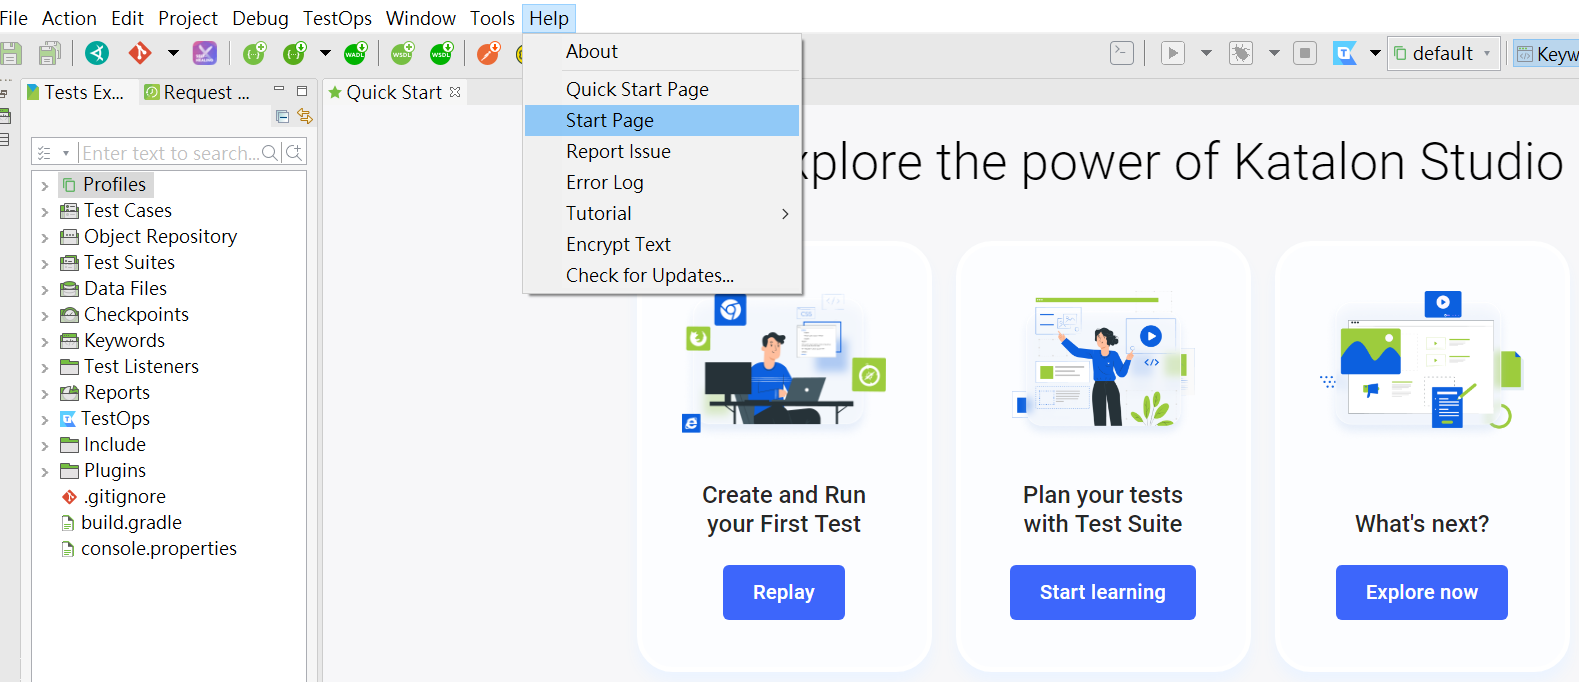
\includegraphics[width=1\textwidth]{picture/quickStart.png}
\end{frame}
%----------------------------
\begin{frame}
    \frametitle{Quick Start}
    由教學可以整理出簡單的結論與順序:
    \begin{enumerate}
        \item 創建 Request 物件,包含設定 URL、Header、Body、自訂變數等
        \item 建立 Test Case Script,將 Request 物件加入
        \item 於 Script 中撰寫驗證規則
        \item 將各 Test Case 組成 Suites 執行
        \item 或再將 Test Case Suites 組成 Collection 執行
        \item 若有失敗發生再將結果輸出報告觀察
    \end{enumerate}
\end{frame}
%----------------------------
\ifx\allfiles\undefined
\end{document}
\fi